\documentclass{article}
\usepackage{caption}
\usepackage{algorithm2e}
\usepackage{authblk}
\usepackage{graphicx}
\usepackage{listings}
\usepackage{array}
\usepackage{courier}
\usepackage{csquotes}
\usepackage[USenglish]{babel}
\usepackage{nameref}

\usepackage[backend=bibtex,sorting=none]{biblatex}
\addbibresource{manuscript}
\graphicspath{{assets/images/}}
\emergencystretch=1em
\DeclareUnicodeCharacter{2212}{-}

\def\ttt{\texttt}

\begin{document}

\hyphenation{organo-metallics Proto-SMILES}
\newcolumntype{L}{>{\arraybackslash}m{3cm}}
\lstset{basicstyle=\ttfamily,breaklines=true}


\title{Dialect: A Compact Line Notation Based on SMILES}
\author{Richard L. Apodaca\thanks{rapodaca@metamolecular.com}}

\maketitle

\section*{Introduction}

Simplified Molecular Input Line Entry System (SMILES) was first described by Weininger in 1988~\cite{weininger:1988}. As a line notation~\cite{wiswesser:1968}, SMILES represents molecules as single line character sequences, or strings. SMILES has since been widely adopted. Read and write functionalities are routinely supported by popular cheminformatics toolkits, including: Open Babel~\cite{oBoyle:2011}; RDKit~\cite{rdkit}; Chemistry Development Kit~\cite{steinbeck:2003}; JChem Base~\cite{jchemBase}; the Daylight Toolkit~\cite{daylightToolkit}; and OEChem TK~\cite{oetk}. SMILES encodings can be found in many public-facing databases, including: PubChem~\cite{kim:2016}; ChEBI~\cite{degtyarenko:2007}; ZINC~\cite{irwin:2005}; ChEMBL~\cite{gaulton:2012}; and Wikipedia~\cite{wikipediaCAS}. Raw SMILES strings have been used extensively in machine learning applications~\cite{sousa:2021}. Algorithmic selection of a single SMILES encoding has been used for unique molecular identification~\cite{weininger:1989,oBoyle:2012}. SMILES has also been extended to carry various forms of metadata, as exemplified by Jmol SMILES~\cite{hanson:2016}, CurleySMILES~\cite{drefahl:2011}, BigSMILES~\cite{lin:2019}, and CXSMILES~\cite{cxsmiles}.

Despite the central role that SMILES plays in cheminformatics, public descriptions of the language remain imprecise at best. A 1987 report to the US Environmental Protection Agency by Weininger described a language similar to SMILES, but with important differences~\cite{anderson:1987}. Weininger's 1988 paper offered an overview of the language, but omitted or only partially addressed points crucial to correctly implementing SMILES, including: (1) stereochemical configuration; (2) double bond conformation; (3) the encoding and decoding of \enquote{aromatic} features; (4) the computation of implicit hydrogen count, especially in the context of aromatic features; (5) formal syntax; (6) constraints on quantities such as mass number and charge; and (7) enumeration of error states.

Since 1988, two authoritative sources have attempted to clarify or revise Weininger's 1988 description of SMILES. A 2003 book chapter by Weininger addressed some of the limitations of the paper~\cite{weininger:2003}. The Daylight Theory Manual, a website maintained by SMILES's corporate sponsor, Daylight Chemical Information Systems, Inc. (\enquote{Daylight}), recapitulates previously-published material~\cite{daylightTheory}. The lack of other authoritative sources describing SMILES is consistent with Weininger's reported disinterest in traditional scientific publication~\cite{gasteiger:2018}.

In 2007 a documentation effort that would become known as OpenSMILES began~\cite{openSMILES}. OpenSMILES was conceived as \enquote{a non-proprietary specification for the SMILES language.} Many of the points left open by previous SMILES documentation efforts were addressed. Noteworthy contributions included: the first formal grammar, later adapted to a standard parser toolchain~\cite{denjoed:2010}; many refinements around stereochemistry; and the introduction of \enquote{standard form.} Absent were detailed procedures for assigning and interpreting aromatic features, and a detailed procedure for computing implicit hydrogen count. OpenSMILES also left several points of syntactic and semantic ambiguity unsettled, while introducing extensions of its own.

In 2019 IUPAC announced the SMILES+ initiative~\cite{smilesPlusSpecification}. Noting the limitations of existing SMILES documentation, the SMILES+ effort seeks to \enquote{establish a formalized recommended up-to-date specification of the SMILES format.} SMILES+ took as its starting point the documentation produced by the OpenSMILES project. Efforts to extend this starting point are in progress online through a public repository, but no formal recommendation has to date resulted~\cite{smilesPlusGitHub}.

The lack of a comprehensive SMILES specification has caused several immediate problems. Maintainers of SMILES implementations lack a blueprint for working toward a common set of features and behaviors. At the same time, authors of new SMILES implementations must address ambiguities on an ad hoc basis. The diversity of implementations combined with language underspecification leaves standards bodies with a limited pool of source material upon which to draw. Widespread divergence around the edges of the SMILES language hampers the development of compliance suites, which only amplifies the problems faced by software teams trying to build compliant software. Finally, extensions to SMILES only make sense in the context of a rigorously defined base language.

More broadly, this situation undermines ongoing data integrity efforts underway in other scientific disciplines. For example, the FAIR Guiding Principles identify four qualities essential for extracting maximum utility from published scholarly data: Findability; Accessibility; Interoperability; and Reusability~\cite{wilkinson:2016}. The lack of a well-developed standard means that chemical data sets based on SMILES will suffer in all four areas.

The very notion of a SMILES standard may not be realistic at this point. Today a dozen or more slightly different implementations are in use. None of them can be considered a reference standard. Some have introduced extensions not recognized by the others, contributing to language drift while compounding the already formidable difficulties faced by implementors. Others claim SMILES compatibility while ignoring certain aspects of the documentation that does exist. The Daylight implementation, like some of the others, is distributed under a commercial license that restricts use~\cite{daylightToolkit}, and a publicly-accessible web service operated for many years has been decommissioned~\cite{depictArchive}. Although SMILES may underpin a lot of modern chemical information exchange, the foundations of this system are weathered and showing signs of stress.

This paper attempts to solve these problems with Dialect, a fully-specified language designed as a subset of SMILES. The following sections present Dialect from three perspectives: as a compact system for molecular representation; as a text-based language; and as a specification for software capable of the lossless conveyance of chemical structure information across organizational and temporal boundaries.

\section*{Goals, Design, and Tradeoffs}

Dialect's purpose is to solve the \textit{molecular serialization} problem. Serialization refers to the process of translating a data structure into a format that can be transmitted over a communication channel for later reconstruction. This is useful because it enables general-purpose devices and networks to convey complex pieces of domain-specific information. Receiver and recipient may be separated by time, space, or both. Molecular serialization extends the concept of serialization to molecular structure. Examples of molecular serialization formats other than SMILES include Chemical Markup Language (CML)~\cite{murray-rust:2011}, CDXML~\cite{cdxml}, and CTfile ("molfile")~\cite{ctfileFormats}.

Molecular serialization require careful attention to two complementary rule sets: \textit{syntax} and \textit{semantics}. Syntax defines the set of valid strings for a language, whereas semantics determine the meaning of valid strings. Incomplete specification of either syntax or semantics can lead to data loss and corruption. The semantics for Dialect are complex due to the brevity of its syntax and the inherently complex nature of molecular representation.

As a molecular serialization scheme, Dialect must balance two opposing factors: generality and complexity. If the chemical space Dialect spans is too broad, complete implementation could become impractical due to language complexity. But if the language is made too simple, the chemical space it spans may be of little interest. An important goal for Dialect is therefore to address the most interesting chemical space with the simplest possible syntax and semantics.

Toward this end, Dialect is built on four mutually-exclusive concepts:

\begin{itemize}
\item \textit{Constitution}, the atoms present in a molecule and how they are connected with each other through bonds. Dialect supports elements having two-letter IUPAC designations and all bonding arrangements available through the valence bond model.
\item \textit{Conformation}, the kind of stereoisomerism resulting from restricted rotation about a bond. Dialect support restricted rotation about double bonds leading to alkene isomerism.
\item \textit{Configuration}, the kind of stereoisomerism resulting from the arrangement of neighboring atoms in three-dimensional space. Dialect supports configurations for atoms having tetrahedral symmetry attached to four neighboring atoms.
\item \textit{Delocalization}, a type of bonding in which electrons are shared among three or more atoms, or across a combination of atoms and bonds. Dialect supports a limited form of delocalization operating over paths of alternating single and double bonds.
\end{itemize}

\begin{figure}
\centering
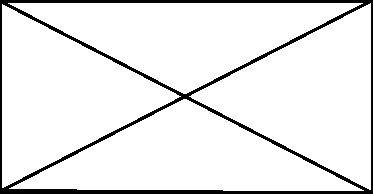
\includegraphics{filler}
\caption{Representative Dialect examples.}
\label{fig:myfig}
\end{figure}

Dialect molecules inherit behavior from an underlying \textit{molecular graph}~\cite{balaban:1985}. A graph is a data structure comprised of a set of nodes and a set of pairwise relationships between them called edges. A molecular graph is a specialized graph onto which chemically-relevant metadata have been overlaid. The presence of this overlay allows nodes and edges to represent atoms and bonds, respectively. Molecular graphs are ubiquitous in cheminformatics, appearing in both serialization formats in-memory data structures found in software toolkits.

A Dialect molecule is a molecular graph having zero or more nodes and zero or more edges. The empty molecule, devoid of atoms and bonds, is therefore allowed. Dialect imposes an upper bound on the number of nodes of $2^{32} - 1$ and the same limit for the number of edges. However, practical limitations related to memory, storage, and CPU time will likely further constrain these limits in practice.

The edges of a Dialect molecular graph are defined as a set of unordered pairs of non-identical nodes. The practical consequences of this are threefold. First, \textit{loops} are not allowed. A loop is an edge joining a node to itself. Second, edges are \textit{undirected}. An undirected edge is equivalent to another edge whose terminals are transposed. With one exception that will be discussed in detail, an undirected edge between nodes A and B is therefore identical to an undirected edge between nodes B and A. Third, \textit{parallel edges} are disallowed. Edges are said to be parallel if they connect the same two nodes.

A molecular graph contains zero or more \textit{connected components}. A connected component is a graph in which any two vertices are connected to each other by at least one path. The maximum number of connected components is equal to the maximum node count, although practical factors may reduce this limit.

\section*{Data Model}

Dialect uses several abstractions collectively known as the \textit{data model}. The data model defines metadata attributes associated with the components of a molecular graph. These attributes are themselves composed of \textit{primitives} (Table~\ref{table:primitives}), or irreducible data types.

\begin{table}
\begin{minipage}{\textwidth}
\renewcommand*\footnoterule{}
\caption{Data Model Primitives.}
\label{table:primitives}
\centering
\begin{tabular}{l l l}
    \hline
    Name & Description & Values\footnote{Ranges defined as \ttt{a..b} include \ttt{a} and exclude \ttt{b}.} \\
    \hline
    \ttt{Option<Type>} & Optional Value & \ttt{None}, \ttt{Type} \\
    \ttt{Index} & Unsigned integer & 0..2\textsuperscript{32} \\
    \ttt{Three} & Integer count & 1..4 \\
    \ttt{Ten} & Unsigned integer & 0..10 \\
    \ttt{SignedTen} & Integer count & -9..10 \\
    \ttt{Thousand} & Integer count & 0..1000 \\
    \ttt{Element} & IUPAC-\-approved element symbol & \ttt{Ac}, \ttt{Ag}, \ttt{Al}, {\ldots}\ttt{Zn}\\
    \ttt{HydrogenCount} & Hydrogen count & \ttt{Implicit}, \ttt{Ten} \\
    \ttt{Configuration} & Configurational descriptor & \ttt{Right}, \ttt{Left} \\
    \ttt{Direction} & Conformational descriptor & \ttt{Up}, \ttt{Down} \\
    \ttt{boolean} & Boolean & \ttt{true}, \ttt{false} \\
    \hline
\end{tabular}
\end{minipage}
\end{table}

An atom possesses several attributes (Table~\ref{table:atomic-state}), which collectively define an \textit{atomic state}. Not all atomic states are valid. Implementations must ensure either the impossibility of an invalid state, or an error condition in the event that one is created. Atomic state is restricted in the following ways:

\begin{table}
\caption{Atomic State.}
\centering
\begin{tabular}{l L L l}
    \hline
    Attribute & Description & Type & Default \\
    \hline
    \ttt{index} & Unique identifier &\ttt{Index} & - \\
    \ttt{element} & Elemental symbol & \ttt{Option} \ttt{<Element>} & \ttt{None} \\
    \ttt{hydrogens} & Hydrogen count & \ttt{HydrogenCount} & 0 \\
    \ttt{configuration} & Configuration & \ttt{Configuration} & \ttt{None} \\
    \ttt{charge} & Formal charge & \ttt{SignedTen} & 0 \\
    \ttt{isotope} & Mass number & \ttt{Option<Thousand>} & \ttt{None} \\
    \ttt{selected} & Selection status & \ttt{boolean} & \ttt{false} \\
    \hline
\end{tabular}
\label{table:atomic-state}
\end{table}

\begin{enumerate}
    \item{The value of \ttt{index} must be unique over the molecular graph.}
    \item{If the value of \ttt{hydrogens} equals \ttt{Implicit}, then the values of \ttt{isotope}, \ttt{configuration}, and \ttt{charge} must equal their respective defaults. Furthermore, the value of \ttt{element} must equal one of \ttt{B}; \ttt{C}; \ttt{N}; \ttt{O}; \ttt{P}; \ttt{S}; \ttt{F}; \ttt{Cl}; \ttt{Br}; \ttt{I}; or \ttt{None}.}
    \item{If the value of \ttt{selected} equals \ttt{true}, then the value of \ttt{element} must equal one of: \ttt{C}; \ttt{N}; \ttt{O}; \ttt{P}; or \ttt{S}.}
\end{enumerate}

Like atoms, bonds carry metadata in the form of attributes (Table \ref{table:bond-state}), which collectively define a \textit{bond state}. As with atomic attributes, not all bond states are valid. Bond state is restricted in the following ways:

\begin{table}
\caption{Bond State.}
\centering
\begin{tabular}{l L L l}
    \hline
    Attribute & Description & Type & Default \\
    \hline
    \ttt{index} & Unique identifier & \ttt{Index} & - \\
    \ttt{source} & Source atom index & \ttt{Index} & - \\
    \ttt{target} & Target atom index & \ttt{Index} & - \\
    \ttt{order} & Bond order & \ttt{Three} & 1 \\
    \ttt{elided} & Elision status & \ttt{boolean} & \ttt{false} \\
    \ttt{direction} & Partial conformational parity & \ttt{Option} \ttt{<Direction>} & \ttt{None} \\
    \hline
\end{tabular}
\label{table:bond-state}
\end{table}

\begin{enumerate}
    \item{The value of \ttt{index} must be unique over the molecular graph.}
    \item{The \ttt{source} and \ttt{target} attributes must reference atomic \ttt{index} attributes found elsewhere in the molecular graph.}
    \item{If the value of \ttt{direction} does not equal \ttt{None}, then the value of \ttt{order} must equal one.}
    \item{If the value of \ttt{elided} equals \ttt{true}, the values of \ttt{order} and \ttt{direction} must equal one and \ttt{None}, respectively.}
\end{enumerate}

The data model will be referenced throughout this paper as a way to connect syntax and semantics. Dialect-compatible software may, of course, use any suitable internal data model. Implementations must, however, ensure that any internal data model is consistent with the one provided here.

\section*{Constitution}

A molecular graph is described at the lowest level by its constitution. In Dialect, constitution comprises the molecular graph and those attributes locating nucleons and electrons at specific atoms and bonds. All other attributes lie outside the scope of constitution. Atomic attributes related to constitution are: \ttt{index}; \ttt{element}; \ttt{hydrogens}; and \ttt{charge}. Bond attributes related to constitution are \ttt{source}, \ttt{target}, \ttt{order}, and \ttt{elided}.

The attributes \ttt{element} and \ttt{isotope} characterize an atom's nucleus. The \ttt{element} attribute is an optional one- or two-letter character sequence selected from the set designated by the IUPAC~\cite{periodicTable}. When IUPAC authorizes additional symbols, they will become valid values for the \ttt{element} attribute. If the elemental identity of an atom is unknown, its \ttt{element} attribute must equal \ttt{None}. The \ttt{isotope} attribute is an optional integer value representing an atom's nuclear mass number, where mass number is the sum of proton and neutron count. Setting the \ttt{isotope} property to \ttt{None} means that the element's isotopic composition equals natural abundance. Otherwise, the lower bound on the value of \ttt{isotope} is zero. This lower limit allows for such physically nonsensical states such as atoms of zero implied mass (\ttt{isotope} equals zero) or negative implied neutron count (e.g., carbon-5). Implementations may reject such atomic states as invalid.

The \ttt{hydrogens} attribute sets an atom's mode of \textit{hydrogen suppression}. Hydrogen suppression replaces an atomic hydrogen of natural isotopic abundance and its associated bond with an integer tally associated with the parent atom. Even so, a suppressed hydrogen and its bond are understood to be present. The relative abundance and regular bonding of hydrogen atoms in molecular graphs makes hydrogen suppression an effective technique for increasing information density. Two mutually-exclusive types of suppressed hydrogen are supported: \textit{virtual hydrogen} and \textit{implicit hydrogen}.

A virtual hydrogen is one that appears as an integer unit contribution associated with the parent atom. For example, methane can be represented by a molecular graph having five nodes and four edges. But methane can also be represented as a graph of one node whose \ttt{hydrogens} attribute equals four. When using this mode, the \ttt{hydrogens} attribute may assume integer values from zero to nine, inclusive. The process of replacing atomic hydrogens with virtual hydrogen is called \enquote{virtualization.} The opposite process, replacing virtual hydrogen with atomic hydrogen, is called \enquote{reification.}

An implicit hydrogen is similar to a virtual hydrogen in that both the hydrogen node and bond have been replaced with a tally. Unlike a virtual hydrogen, however, this tally is not present as attribute on the parent atom but rather as a computation. Subject to certain limitations, an atom identifies itself as having an implicit hydrogen count by setting its \ttt{hydrogens} attribute to \ttt{Implicit}. The computation and its limitations will be described later in this paper.

The atomic attribute, \ttt{charge}, enables electron counting. The purpose of electron counting is to associate each electron in a molecular graph with either an atom or a bond. This is a fundamental requirement for the principle of mass conversion. In a more practical sense, electron counting lays the foundation for calculations of formal charge and bond order~\cite{dietz:1995}.

Electron counting in Dialect is based on the well-known \textit{valence bond model} (VB Model)~\cite{lewis:1916}. Although not commonly considered as such, the VB model can be thought of as an algorithm for molecular assembly. This perspective is especially useful given that Dialect itself can be viewed as a programming language for molecular assembly.

A simplified algorithm for electron counting can be summarized as follows. A molecular graph starts as a set of disconnected atoms and an integer electron count equal to the atomic number of the atom's element. Two nodes are selected as the terminals of a bond. From each atom, the same positive electron count is deducted. The total electron count deducted from each atom is simultaneously credited to the bond's electron count. For example, if each atom contributes one electron to a bond, then the bond's electron count will increase by two.

\begin{figure}
    \centering
    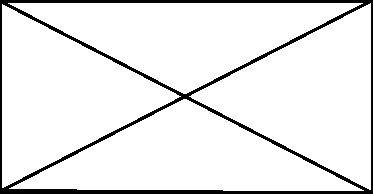
\includegraphics{filler}
    \caption{Generalized Valence Bond Electron Counting. Two unconnected nodes are chosen for bonding (left). One electron is subtracted from each atom, and both electrons are added to the bond's count (right).}
    \label{fig:electron-counting}
\end{figure}

For convenience, the actual model used by Dialect differs slightly from the above description. Neither nodes nor edges carry an explicit electron count attribute. Instead, edges carry an \ttt{order} attribute, and nodes carry a \ttt{charge} attribute. Bond order equals electron count divided by two. Formal charge equals the number of electrons gained or lost due to ionization events outside of bond formation. Gaining an electron decrements the \ttt{charge} attribute, whereas losing an electron increments it. If no electrons are gained or lost to ionization outside of bond formation, the formal charge equals zero. 

\begin{figure}
    \centering
    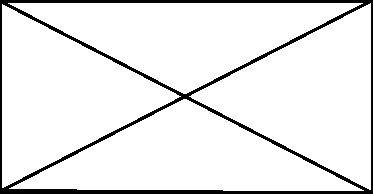
\includegraphics{filler}
    \caption{Electron counting shorthand. Rather than explicit electron counts, atoms and bonds possess charge and order attributes. The atomic charge attribute captures deviations from generalized counting.}
    \label{fig:electron-counting-shorthand}
\end{figure}

From these rules follow some practical consequences. For one, bond order must be an integer greater than zero. This follows from the definition of bond formation. The electron count deducted from each atom is $n$, an integer greater than zero. Given that bond formation deducts an equal number of electrons from each atom, the total number of electrons associated with the newly-formed bond is $2n$. By definition, bond order is the bond's electron count divided by two, therefore $n$ is the bond order. Fractional, negative, and zero bond orders are all disallowed by Dialect for this reason.

Dialect imposes an upper limit of three on formal bond order. The relative scarcity of bond orders greater than this limit in molecules conforming the the VB Model makes this restriction unlikely to meaningfully restrict applicability.

Whereas negative bond order is disallowed by definition, Dialect places no restrictions on \textit{hypervalence}. Hypervalence occurs when an atom undergoes enough bonding operations to leave it with a negative implied valence electron count. Consider lithium, which possesses one valence electron. Formation of one single bond leaves lithium with zero implied valence electrons. Application of a second bond formation leaves lithium with a zero charge and an implied valence electron count of -1. Such an arrangement may be physically meaningless, but Dialect explicitly supports it. Software using Dialect may or may not reject such species for semantic reasons.

\begin{figure}
    \centering
    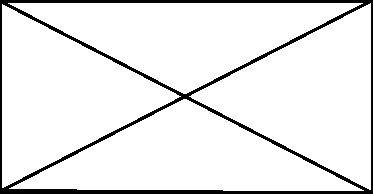
\includegraphics{filler}
    \caption{Hypervalence. Depletion of atomic electron count through excessive bonding. Hypervalent atoms are valid by default, although chemically nonsensical.}
    \label{fig:hypervalence}
\end{figure}

Each atom carries an \ttt{index} attribute, allowing bonds to reference atoms in a molecular graph. To do so, the \ttt{source} and \ttt{target} attributes are set with the respective indexes of the source and target atoms. The set of all bonds and the nodes they reference determines the connectivity of a molecular graph. In the context of determining connectivity, source and target indexes may be reversed.

\section*{Bond Elision}

A bond whose attributes are assigned default values can participate in \textit{bond elision}. In bond elision, a bond's \ttt{elided} attribute is set to \ttt{true}. When written in string form, elided bonds require no characters. This makes bond elision useful for data compression. The second application for elided bonds will be described in the next section.

\section*{Delocalization Subgraph}

A molecular representation based solely on the valence bond model can yield artifacts resulting from \textit{delocalization induced molecular equality} (DIME). DIME arises when a molecular graph exists in two or more unequal forms, each differing from the others only through electron delocalization. In this context, two graphs are equal if they are isomorphic and each matched pair of atoms or bonds possess equivalent non-index attributes. If shifting electrons through delocalization causes two graphs to become equal, then DIME has occurred. DIME is sometimes referred to as \enquote{resonance} or \enquote{aromaticity,} but those terms are avoided here due to their ambiguity~\cite{randic:2018,kerber:2006}.

\begin{figure}
    \centering
    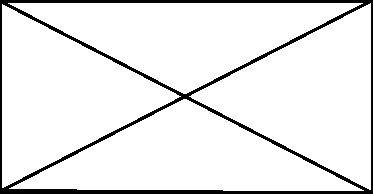
\includegraphics{filler}
    \caption{Delocalization-induced molecular equality (DIME). Two chemically equivalent molecular graphs differ on the basis of delocalization.}
    \label{fig:dime}
\end{figure}

DIME can interfere with \textit{canonicalization}, or the selection of a single representation for a molecular graph. The presence of multiple equivalent molecular graphs differing only in electron delocalization complicates the formulation of selection rules and invariants, which must be adapted to account for the artificial asymmetry.

To eliminate DIME and thereby streamline canonicalization, the molecular graph is augmented with a \textit{delocalization subgraph} (DS). A DS is a possibly empty node-induced subgraph of a molecular graph. The membership of a DS may be drawn from the set of atoms and bonds that participate in DIME within a given molecular graph.

Membership of a DS is determined as follows. An atom is added to the DS by setting its \ttt{selected} attribute to \ttt{true} through a process called \textit{selection}. For an atom to be selectable, its \ttt{element} attribute must be contained in the list: \ttt{C}; \ttt{N}; \ttt{O}; \ttt{P}; and \ttt{S}. Atoms having other elements must not be selected. A bond will be added to the DS if both of its terminals are selected and the \ttt{elided} attribute equals \ttt{true}. No other bond will be added to the DS. This rule allows arbitrary bonds between selected atoms to be excluded from the DS.

Atoms whose \ttt{element} attribute equals \ttt{None} are not selectable, which prevents their entry into the DS. Bonds to such atoms are similarly excluded. The alternative, conditional inclusion, would complicate both data structures and algorithms for little gain. Exclusion avoids these complexities.

\begin{figure}
    \centering
    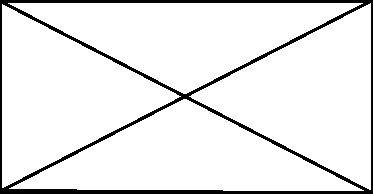
\includegraphics{filler}
    \caption{Perfect Matching. A subgraph with all of the nodes of its parent, but in which all nodes have degree one.}
    \label{fig:perfect-matching}
\end{figure}

A non-empty DS must possess a \textit{perfect matching}. A matching is a subgraph in which no two edges share a common node. Equivalently, a matching is a subgraph in which all nodes have degree one. A perfect matching includes all the nodes of its parent graph. Every atom added to a DS must therefore become part of its perfect matching.

A filled DS can be emptied through a two-step process of \textit{deselection}. First, a perfect matching over the DS is found. Next, each matched edge is replaced by a double bond. Because the presence of a filled DS implies a perfect matching over it, kekulization always succeeds. A widely-used algorithm for matching, the Edmunds \enquote{blossom algorithm,} has a time complexity of $O(|E||V|^2)$, where $|E|$ is the number of edges and $|V|$ is the number of nodes~\cite{edmonds:1965}. Although more efficient algorithms are known, they are either much more difficult to implement or lack generality.

\begin{figure}
    \centering
    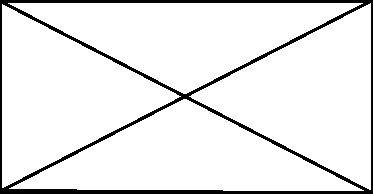
\includegraphics{filler}
    \caption{Deselection. Unsetting the atomic selected flag with simultaneous promotion of matching bonds.}
    \label{fig:deselection}
\end{figure}

The opposite operation can be accomplished with a \textit{selection algorithm}. A selection algorithm selects two or more atoms, thereby adding them to the DS. The only requirement for a selection algorithm is that the resulting DS must have a perfect matching. Depending on the application, other criteria may be applied. For example, a selection algorithm may restrict candidate atoms to those found in cycles. Electron-counting techniques may also be introduced to approximate the chemical concept of \enquote{aromaticity.} Elision of the single bonds to be added to the DS completes the process.

\begin{figure}
    \centering
    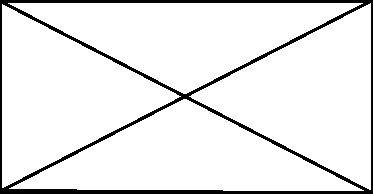
\includegraphics{filler}
    \caption{Selection Algorithm. Those atoms with bonds contributing to DIME are added to the delocalization subgraph.}
    \label{fig:selection}
\end{figure}

\section*{Valence and Subvalence}

To support implicit hydrogen counting, Dialect uses the concept of \textit{valence}. Valence is a non-negative integer computed as the sum of bond orders at a given atom. Single and elided bonds contribute one to the tally, double bonds two, and triple bonds three. Each virtual hydrogen contributes one. For example, the valence of a methyl carbon having three virtual hydrogens and a hydrogen neighbor is four. The valence of an acetaldehyde oxygen atom is two. And so on.

Some elements are associated with one or more \textit{default valences} (Table~\ref{table:default-valences}). A default valence is the number of hydrogens that can be attached to an isolated, fully-saturated atom using the corresponding element. For example, the default valence for a carbon-bearing atom is 4. This means that a fully saturated atom of carbon will have four hydrogens. Likewise, a fully-saturated atom of oxygen will have two hydrogens. Some elements such as nitrogen are associated with multiple default valences. In these cases, multiple saturated forms are possible. For example, nitrogen has the default valences three and five. Both ammonia (NH\textsubscript{3}) and nitrogen pentahydride (NH\textsubscript{5}) are therefore fully saturated forms of nitrogen according to Table~\ref{table:default-valences}.

\begin{table}
    \caption{Default Valences.}
    \centering
    \begin{tabular}{l l}
        \hline
        Element & Valences \\
        \hline
        B & 3 \\
        C & 4 \\
        N & 3,5 \\
        O & 2 \\
        F & 1 \\
        P & 3,5 \\
        S & 2,4,6 \\
        Cl & 1 \\
        Br & 1 \\
        I & 1 \\
        \hline
    \end{tabular}
    \label{table:default-valences}
\end{table}

Given an atom whose element has one or more default valences, \textit{subvalence} can be computed. Subvalence is the number of hydrogens that can be added to an atom without exceeding the lowest possible default valence. If no suitable default valence exists, then subvalence equals zero. This computation can be expressed algorithmically (Algorithm~\ref{algorithm:subvalence}). First, the atom's valence is computed. Next, the ordered list of default valences of the atom's element is found. For each default valence, the difference between it and the valence is compute. If this differences is positive, it is returned as the subvalence. If no suitable default valence is found, zero is returned. The subvalence of an atom whose element has no default valences (i.e., no listing in Table~\ref{table:default-valences}) is zero. For example, an iron atom always has a subvalence of zero, regardless of how it is bonded.

\begin{algorithm}
    \SetKwInOut{Input}{input}
    \SetKwInOut{Output}{output}
    \SetKwFunction{BondOrderSum}{BondOrderSum}
    \SetKwFunction{TargetValences}{TargetValences}
    \caption{Computing subvalence.}
    \label{algorithm:subvalence}
    
    \Input{An atom $a$ with one or more default valences}
    \Output{The subvalence of $a$}
    \Begin{
      $v \leftarrow$ Valence($a$)\;
      $T \leftarrow$ DefaultValences($a$)\;
      \For{$t \in T$}{
        $d \leftarrow t-v$\;
        \If{$d >= 0$}{
          \Return{$d$}\;
        }
      }
      \Return{$0$}\;
    }
\end{algorithm}

For a representative subvalence computation, consider an isolated nitrogen atom without virtual hydrogens. The atom's bond order sum is zero. Its default valences are 3 and 5. The difference is found to be three ($3 - 0$). Therefore, the subvalence of this atom is three.

The carbonyl carbon atom of acetaldehyde illustrates the effects of substitution and multiple bonding. Bond order sum is three (2 + 1). From Table~\ref{table:default-valences}, default valence is four. Subtracting bond order sum from default valence yields one ($4 - 3$), which is returned as the atom's subvalence.

The phosphorous atom in phosphorous acid (H\textsubscript{3}PO\textsubscript{3}) illustrates the use of Algorithm \ref{algorithm:subvalence} for atoms with multiple target valences. Bond order sum is four ($2 + 1 + 1$). The first default valence is 3, but subtracting valence from that value yields a negative number ($3 - 4$). Continuing to the next default valence, five, a difference of 1 is obtained. Therefore, the subvalence of the phosphorous-bearing atom is reported as one.

The valence of some atoms exceeds the largest default valence. In these cases, subvalence is reported as zero. Consider sodium perchlorate (NaClO\textsubscript{4}). The chlorine atom has a bond order sum of seven ($2 + 2 + 2 + 1$). From Table~\ref{table:default-valences}, the only default valence for chlorine is one. Subtracting seven yields a negative number (-6). Therefore, the subvalence is reported as zero.

\section*{Computing Implicit Hydrogen Count}

An atom whose \ttt{hydrogens} attribute equals \ttt{Implicit} signals that its hydrogens must be counted algorithmically. The exact algorithm depends on the value of the atoms's \ttt{selected} attribute.

For an unselected atom, implicit hydrogen count equals subvalence. For example, an oxygen atom with one single bond has an implicit hydrogen count of one because subvalence is one ($2 - 1$). Similarly, an oxygen atom with two singly-bonded neighbors has an implicit hydrogen count of zero ($2 - 2$).

For a selected atom, implicit hydrogen count equals subvalence minus one. This subtraction accounts for the extra valence implied by the atom's membership in the delocalization subgraph. Consider a selected carbon atom in benzene with a \ttt{hydrogens} attribute of \ttt{Implicit}. Subvalence equals two ($4 - 2$), so implicit hydrogen count equals one ($2 - 1$). Likewise, the subvalence of a selected nitrogen atom in pyridine equals one ($3 - 2$) so implicit hydrogen count equals zero ($1 - 1$). Stated differently, the calculation ensures that an atom's implicit hydrogen count is identical before and after deselection.

If the subvalence of a selected atom equals zero, then an implicit hydrogen count of zero is reported. The meaning of such an atomic state may seem suspect because an atom without a free valence can not perform the required promotion of a single bond during deselection. As will be explained in detail later (Pruning), this situation can arise for reasons of convenience or tradition. Returning zero avoids miscalculation of the implicit hydrogen count.

An atom's implicit hydrogen count may or may not correlate with chemical intuition or experimental data. Consider the phosphorous-bearing atom of hypophosphorous acid (HOP(O)H\textsubscript{2}). We might expect the implicit hydrogen count to equal the experimentally-determined hydrogen count (2). However, the subvalence for the phosphorous atom is found to be three ($2 + 1 - 3$). The implicit hydrogen count is therefore zero ($3 - 3$) rather than the expected two. To represent this atom and other like it, virtual hydrogens must be used.

\begin{figure}
    \centering
    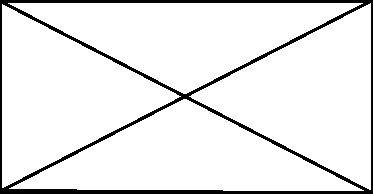
\includegraphics{filler}
    \caption{Implicit hydrogen count. The number of hydrogens is set algorithmically.}
    \label{fig:implicit-hydrogen-count}
\end{figure}

\section*{Atom Index}

To support the assignment and interpretation stereochemical features, each node carries a unique, non-negative integer \ttt{index} attribute (\enquote{index}). Assignment is sequential, meaning that the first atom gets index zero, the next one, and so on. For example, the index for the first atom is zero, for the second atom one, for the third atom two, and so on. The maximum value of an atomic index is 2\textsuperscript{32} - 1.

Indexes impose an ordering over the atoms in a molecular graph. An atom with an index less than another atom is said to \textit{precede} it. An atom with an index grater than another atom \textit{succeeds} it. No special significance is ascribed to the atom whose index is zero, except that every other atom succeeds it.

\section*{Conformation}

The second major component of molecular representation in Dialect is \textit{conformation}. Conformation is a rotational restriction about one or more bonds. Dialect limits conformation to just one of many possible types: rotational restrictions occurring at individual double bonds.

Organic chemistry uses the descriptors \textit{entgegen} (\textit{E}) and \textit{zusammen} (\textit{Z}) to label conformational parity. This system is based on prioritization of the atoms neighboring the double bond. One pattern of priority yields the \textit{E} parity, and the other yields \textit{Z}. Conveniently, the parity descriptor can be localized at the double bond.

\begin{figure}
    \centering
    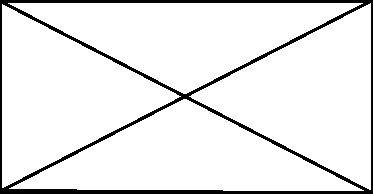
\includegraphics{filler}
    \caption{Traditional conformational stereodescriptors.}
    \label{fig:traditional-conformational-stereodescriptors}
\end{figure}

Dialect takes a different approach by introducing \textit{partial parity bonds} (PPB). As the name implies, a PPB expresses a portion of the parity characterizing a conformationally-restricted double bond. Constructing the full parity requires the double bond itself, and at least two PPBs. With just a few exceptions (see below), a double bond with a neighbor at one terminal bound through a PPB must also have a neighbor at the opposite terminal bound through a PPB.

\begin{figure}
    \centering
    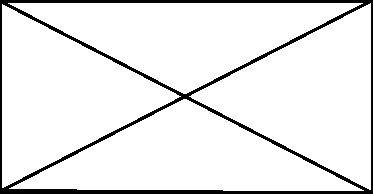
\includegraphics{filler}
    \caption{Partial parity bond. Bond conformational parity is distributed over two or more bonds.}
    \label{fig:partial-parity-bonds}
\end{figure}

To support this system, each bond carries an optional \ttt{direction} attribute (\enquote{direction}). When present, direction may assume one of the two values \ttt{Up} or \ttt{Down}. These values refer to a geometrical model in which the two terminals of a double bond and their neighbors are assigned local relative coordinates in a plane. The terminals of the bond are placed on the x-axis such that the one on the right succeeds the one on the left. The neighbors at each terminal joined through a PPB are then assigned relative coordinates in the plane.

Neighbors of the left terminal are positioned according to the relative ordering of atomic indexes and the bond's \ttt{direction} attribute. If the neighbor precedes the terminal then a \ttt{direction} attribute equal to \ttt{Up} locates the neighbor in the lower-left quadrant and a \ttt{direction} attribute of \ttt{Down} locates the neighbor in the upper-left quadrant. If the neighbor succeeds the terminal, these placements are reversed.

An analogous procedure assigns relative coordinates to a neighbor of the right terminal. If a neighbor succeeds the right terminal, place it to the upper right given an \ttt{Up} direction, or to the lower right given a \ttt{Down} direction. Reverse these assignments if the neighbor precedes the right terminal.

\begin{figure}
    \centering
    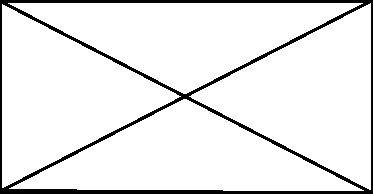
\includegraphics{filler}
    \caption{Interpreting partial parity bonds.}
    \label{fig:interpret-ppb}
\end{figure}

In some cases the placement of a terminal neighbor can be deduced from the placement of a sibling, without the presence of an explicit PPB. For example, a left terminal has two neighbors, but only one of them uses a PPB. The neighbor with the PPB can then be placed explicitly. Doing so allows the remaining neighbor without a PPB to be placed as well by elimination. For example, if the neighbor of a left terminal is placed in the upper left quadrant, then the sibling without a PPB can only occupy the lower left quadrant.

\begin{figure}
    \centering
    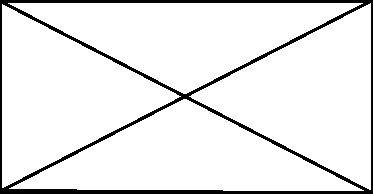
\includegraphics{filler}
    \caption{Implied neighbor placement. Bond directions can be omitted when inferrable.}
    \label{fig:implied-neighbor-placement}
\end{figure}

The assignment of relative coordinates to both terminals and all neighbors yields a double bond conformation.

Consider the encoding of PPBs for (\textit{E})-2-butene. Assume that indexes are assigned sequentially from the neighbor of the left terminal to the neighbor of the right terminal and that the goal is to arrive at a trans (or anti) substituent orientation. Begin by placing the two double bond terminals on the x-axis according to succession. The left terminal succeeds its neighbor, which should be placed in the lower-left quadrant. To achieve this, assign a PPB direction of \ttt{Up}. The right terminal precedes its neighbor, which should be placed in the upper-right quadrant. To active this, assign a PPB direction of \ttt{Up}.

\begin{figure}
    \centering
    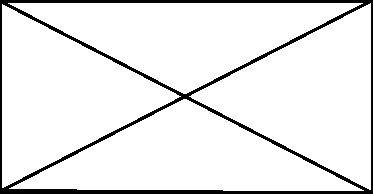
\includegraphics{filler}
    \caption{Assigning partial parity bonds to *trans*-2-butene.}
    \label{fig:assigning-ppb}
\end{figure}

PPBs are decoded analogously. Start by placing the terminals on the x-axis according to succession. The PPB between the left terminal and its neighbor has a direction of \ttt{Up}. Because the neighbor precedes the terminal, the neighbor should be placed in the lower-left quadrant. The PPB between the right terminal and its neighbor has a direction of \ttt{Up}. Because the neighbor succeeds the terminal, the neighbor is placed in the upper-right quadrant. The result is the expected (\textit{E}) conformation.

The above procedures assume that all PPBs are expressed in \textit{normal form}. In normal form, a PPB's source precedes it target. In other words, \ttt{source} is less than \ttt{target}. If a PPB is not in normal form, it must be \textit{inverted} before quadrants can be assigned. Inversion swaps the values of `source` and target attributes while simultaneously toggling the `direction` attribute. Inversion occurs in two contexts: conjugated polyenes and cycles. In the case of polyenes, the same PPB carries partial conformation for at least two different double bond systems. In the case of cycles, non-normal PPBs can be generated at bonds forming cycles. However, readers and writers must be capable of inverting PPBs wherever they appear.

\begin{figure}
    \centering
    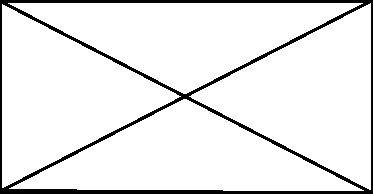
\includegraphics{filler}
    \caption{Partial parity bond inversion. Direction must be inverted for bonds not expressed in normal form.}
    \label{fig:ppb-inversion}
\end{figure}

The distributed nature of conformational encoding means that several additive error states are possible:

\begin{itemize}
    \item{Overspecification. This state occurs when two or more PPBs share a common terminal and simultaneously use the same parity, thus placing multiple neighbors into the same quadrant.}
    \item{Underspecification. A required and non-deducible PPB is absent. This state occurs when a double bond terminal connects to at least one neighbor through a PPB, but the terminal's mate does not.}
    \item{ Misspecification. A PPB is used between atoms lacking at least one double bond.}
\end{itemize}

A reader that detects one of these error conditions must abort the molecular graph being read and report the error state. It is possible for a conformation to be both overspecified and underspecified.

\begin{figure}
    \centering
    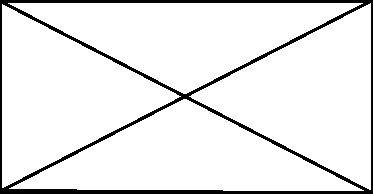
\includegraphics{filler}
    \caption{Error bond states. Because conformational descriptions are defined over three or more bonds, a variety of error states are possible.}
    \label{fig:bond-error-states}
\end{figure}

An exception to the underspecification rule applies in the case of conjugated polyenes. Here a double bond with a terminal connected through a PPB does not require the opposing terminal to also bear a neighbor connected through a PPB. If the opposing terminal lacks neighbors, no error is generated and reading continues normally. If the opposing terminal has at least one neighbor, the bond to it need not be a PPB. In either case the conformation of the double bond in question remains undefined.

\begin{figure}
    \centering
    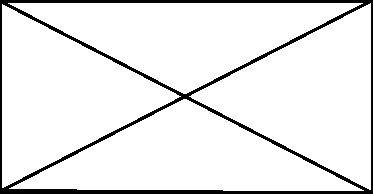
\includegraphics{filler}
    \caption{Error state exceptions. Conjugated dienes sharing a common PPB can lead to exceptional cases.}
    \label{fig:bond-error-state-exceptions}
\end{figure}

Given that conformational specification is distributed over three or more bonds, some conformations will be difficult or possible to represent. Cyclooctatetraene offers an example. Although the (\textit{E}, \textit{E}, \textit{E}, \textit{E}) conformation is expressable, the (\textit{Z}, \textit{E}, \textit{E}, \textit{E}) conformation is not. This problem arises because the same PPB encodes a partial conformation of two different double bonds.

\begin{figure}
    \centering
    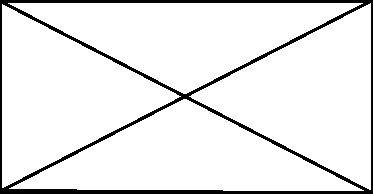
\includegraphics{filler}
    \caption{Cyclooctatetraene. Some double bond conformations are not expressable.}
    \label{fig:cyclooctatetraene}
\end{figure}

\section*{Configuration}

The third major element of molecular representation is \textit{configuration}, the three-dimensional arrangement of neighbors about a central atom. Dialect limits configuration to the special case of an atom with exactly four substituents placed at the vertices of a tetrahedron. Here, \enquote{substituent} means an atomic neighbor or virtual hydrogen. Lone electron pairs are not considered substituents.

A configuration is comprised of two components: an ordering of bonds to a central atom; and a \textit{configurational descriptor}. A configurational descriptor is a template for the relative three-dimensional positioning of neighbors about a central atom. Dialect supports two configurational descriptors: \ttt{Left} and \ttt{Right}. These descriptors constrain the neighbors of a central atom to the vertices of a tetrahedron.

The \ttt{Left} variant works as follows. First, the bond having the index with the lowest value identified. The frame of reference is shifted by sighting down this bond from the neighbor to the central atom. An equilateral triangle with one vertex pointing upward is then inscribed about the central atom. The bond with the next lowest index is then identified and its neighbor is placed at the top vertex of the triangle. The neighbor attached to the succeeding bond is then placed at the left triangle vertex. Finally, the remaining neighbor is placed at the remaining vertex. The overall pattern is one of counterclockwise distribution.

The \ttt{Right} variant follows the same pattern, except that placement of the neighbors attached to the last two bonds in succession are transposed. The overall pattern here is one of clockwise distribution.

\begin{figure}
    \centering
    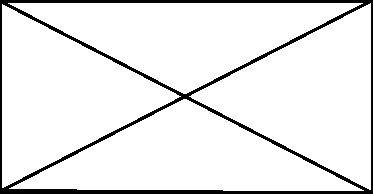
\includegraphics{filler}
    \caption{Configurational descriptor. Configuration is either encoded or reconstructed using the same model.}
    \label{fig:configurational-descriptor}
\end{figure}

A modified procedure is used for atoms bearing one virtual hydrogen and three atomic substituents. The implied bond to the virtual hydrogen is considered to precede the others. Sighting down this bond, the atomic neighbors are then placed as previously at the vertices of a triangle inscribed about the central atom.

\begin{figure}
    \centering
    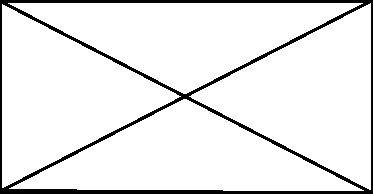
\includegraphics{filler}
    \caption{Configurational descriptor with one virtual hydrogen. In this case, hydrogen assumes the role of the first substituent.}
    \label{fig:configurational-descriptor-vh}
\end{figure}

An atom whose \ttt{configuration} attribute assumes a non-default value must have a neighbor count of either four if no virtual hydrogens are present or three if one virtual hydrogen is present. In any other context, the use of a configurational descriptor is considered an error.

This restriction places some constraints around the use of configuration. Some topologies may appear close enough to tetrahedral to stretch the meaning of the configurational descriptors. However, all such adaptations are invalid. Examples include the central atom of allenes and other odd cumulenes, and the sulfur atom of sulfoxides where the lone pair plays the role of a substituent.

\begin{figure}
    \centering
    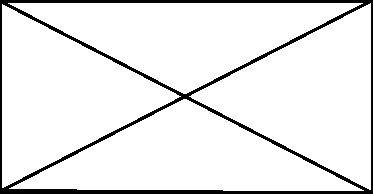
\includegraphics{filler}
    \caption{Invalid uses of configurational descriptors. Only configuration about four-coordinate tetrahedral atoms is supported.}
    \label{fig:invalid-configurational-descriptors}
\end{figure}

A configurational descriptor may be applied without regard to bond type. In other words, single, double, triple, and partial parity bond types can all be present. The only requirement that must be satisfied by a central atom is a neighbor count of four, or three when a virtual hydrogen is present.

It is sometimes useful to manipulate a configuration in a way that preserves the relative three-dimensional positioning of neighbor atoms. This process is called \textit{transformation}. Five operations suffice to transform any configuration into any other:

\begin{itemize}
    \item{Virtualize. Replaces an atomic hydrogen neighbor with a virtual hydrogen. If the deleted bond was first in the bond ordering, toggle the configurational descriptor.}
    \item{Reify. Replaces a virtual hydrogen with an atomic hydrogen neighbor. The bond ordering must place the new neighbor in the second position.}
    \item{Swap. Exchanges any two bonds ordered second or higher while simultaneously toggling the configurational descriptor.}
    \item{Slide Left. Re-orders a bond from the first position to the second position. Disabled if the central atom carries a virtual hydrogen.}
    \item{Slide Right. Re-orders a bond from the second position to the first position. Disabled if the central atom carries a virtual hydrogen.}
\end{itemize}

\begin{figure}
    \centering
    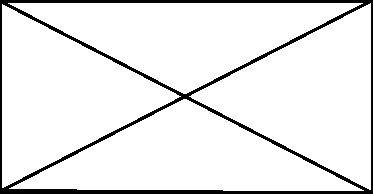
\includegraphics{filler}
    \caption{Configurational Transformations.}
    \label{fig:iconfigurational-transformations}
\end{figure}

Not all tetracoordinate atoms will be \textit{stereocenters}. A stereocenter is an atom whose \enquote{ligand permutation produces stereoisomers,} as defined by Mislow and Siegel~\cite{mislow:1984}. In the context of Dialect, a stereocenter must be tetracoordinate. However, this is a necessary but insufficient condition. Molecular topology can result in permutation that does not produce stereoisomers. Readers should avoid the assignment of stereodescriptors to atoms that are not stereocenters.

Special handling is required for \textit{undefined stereocenters}. A stereocenter is undefined if it lacks a stereodescriptor. Omitting a stereodescriptor conveys to readers that no information about the stereocenter's configuration is known. This could imply that either a single configuration or a configurational mixture are present. This interpretation is consistent with the one used by molfile format~\cite{ctfileFormats}.

\section*{Syntax}

A Dialect string is a UTF-8-encoded sequence of zero or more characters chosen from the set \{ \ttt{A}, \ttt{B}, \ttt{C}, \ttt{D}, \ttt{E}, \ttt{F}, \ttt{G}, \ttt{H}, \ttt{I}, \ttt{K}, \ttt{L}, \ttt{M}, \ttt{N}, \ttt{O}, \ttt{P}, \ttt{R}, \ttt{S}, \ttt{T}, \ttt{U}, \ttt{V}, \ttt{W}, \ttt{X}, \ttt{Y}, \ttt{Z}, \ttt{a}, \ttt{b}, \ttt{c}, \ttt{d}, \ttt{e}, \ttt{f}, \ttt{g}, \ttt{h}, \ttt{i}, \ttt{k}, \ttt{l}, \ttt{m}, \ttt{n}, \ttt{o}, \ttt{p}, \ttt{r}, \ttt{s}, \ttt{t}, \ttt{u}, \ttt{v}, \ttt{0}, \ttt{1}, \ttt{2}, \ttt{3}, \ttt{4}, \ttt{5}, \ttt{6}, \ttt{7}, \ttt{8}, \ttt{9}, \ttt{+}, \ttt{-}, \ttt{.}, \ttt{\%}, \ttt{@}, \ttt{*}, \ttt{[}, \ttt{]}, \ttt{/}, \ttt{\char`\\}, \ttt{=}, \ttt{\#} \}. The internal structure of a string reflects a depth-first traversal of the corresponding molecular graphs. As such, the syntax supports branches, cycles, and disconnected components.

Strings conform to an \textit{LL(1) grammar}.\cite{thain:2020} An LL(1) grammar is a context-free grammar whose strings can be parsed one character at a time from left to right with at most one character of lookahead. Additionally, LL(1) grammars expand the leftmost non-terminal first. These features make LL(1) grammars such as the one used by Dialect a good fit for manually-written recursive descent parsers. LL(1) grammars can also be used as a basis for auto-generated parsers through packages such as ANTLR~\cite{parr:2014}. The full grammar for Dialect strings is available as a text file in this paper's Supporting Material.

Dialect's formal grammar is presented as a series of \textit{production rules} (aka \enquote{productions}). A production rule defines a transformation allowed under the grammar. These transformations collectively define the set of valid Dialect strings. Production rules can be used in the forward direction, when writing a string, or in the reverse direction, when reading a string. 

A production rule is composed of two kinds of elements: \textit{terminals} and \textit{non-terminals}. A terminal is a character literal (e.g., \enquote{A}). A non-terminal is a reference to another production rule. This reference occurs through a name, which appears to the left of a separator (\ttt{::=}) in a production rule. To the right of a separator appear the allowed terminals and non-terminals for the rule.

Consider a hypothetical language composed of variable-length sequences of the lowercase letter \enquote{a}. Such a language could be cast as the following two production rules:

\begin{lstlisting}
<text> ::= <a>*
<a>    ::= "a"
\end{lstlisting}

The quantifier (\ttt{*}) indicates that a text in this language consists of a sequence of zero or more instances of the production \ttt{<a>}. This production in turn is defined as a lowercase letter (\enquote{a}). Therefore, valid texts in this language include the empty string, \enquote{a}, \enquote{aa}, and \enquote{aaaaaa} to name a few.

\subsection*{Atom}

Atoms carry most of the information in a Dialect string. The non-terminal \ttt{<atom>} can be expressed using one of four variants.

\begin{lstlisting}
<atom> ::= <star> | <shortcut> | <selection> | <bracket>
\end{lstlisting}

The first variant, \ttt{<star>}, produces one terminal value, the asterisk character (\ttt{*}). This \enquote{star atom} represents an atom in which every attribute assumes its default value.

\begin{lstlisting}
<star> ::= "*"
\end{lstlisting}

The next atomic production rule, \ttt{<shortcut>} is a non-terminal selected from the list: \enquote{B}; \enquote{C}; \enquote{N}; \enquote{O}; \enquote{P}; \enquote{S}; \enquote{F}; \enquote{Cl}; \enquote{Br}; and \enquote{I.} An atom encoded in this way (\enquote{shortcut atom}) receives the corresponding symbol as the value for the \ttt{element} attribute. All other attributes retain their default values, except \ttt{hydrogens}, which is set to \ttt{Implicit}.

\begin{lstlisting}
<shortcut> ::= "B" "r"? | "C" "l"? | "N" | "O" | "P"
             | "S" | "F" | "I"
\end{lstlisting}

The third atomic production rule, \ttt{<selection>} is a non-terminal selected from the list: \enquote{c}; \enquote{n}; \enquote{o}; \enquote{p}; and \enquote{s.} An atom encoded in this way (\enquote{selected shortcut atom}) assigns the corresponding atom symbol to the \ttt{element} attribute, sets the \ttt{selected} attribute to \ttt{true}, and sets the \ttt{hydrogens} attribute to \ttt{Implicit}. All other atomic attributes retain their default values.

\begin{lstlisting}
<selection> ::= "c" | "n" | "o" | "p" | "s"
\end{lstlisting}

The fourth and most complex atomic production rule is \ttt{<bracket>} (\enquote{bracket atom}). Bracket can be used to set any atomic attribute. A bracket atom must be used for any atom whose \ttt{configuration}, or \ttt{charge} attributes deviate from default values, or whose \ttt{hydrogens} attributes equals anything other than \ttt{Implicit}. Attributes not set within the \ttt{<bracket>} production rule will leave the corresponding atomic values in their default states.

\begin{lstlisting}
<bracket> ::= "[" <isotope>? <symbol> <stereodescriptor>?
              <virtual_hydrogen>? <charge>? "]"
\end{lstlisting}

The value of a bracket atom's \ttt{isotope} attribute is determined by the optional \ttt{<isotope>} non-terminal. It consists of between one and three digits encoding the integers 0-999. Leading zeros are disregarded when assigning the value of the \ttt{isotope} attribute. In other words, \enquote{007} and \enquote{7} are considered equivalent expressions of the value 7.

\begin{lstlisting}
<isotope> ::= <digit> <digit>? <digit>?
\end{lstlisting}

The values of a bracket atom's \ttt{element} and \ttt{selected} attributes are determined by the \ttt{<symbol>} production rule (\enquote{symbol}). Three non-terminal variants are supported. These three variants influence the \ttt{element} and \ttt{selected} attributes in different ways. The \ttt{<star>} variant leaves both attributes as their default values. The \ttt{<element>} variant assigns the \ttt{element} attribute to the corresponding value while leaving the \ttt{selected} attribute as its default value. The \ttt{<selection>} non-terminal sets the \ttt{element} attribute to the corresponding element and the \ttt{selected} attribute to \ttt{true}. For example, the selection sequence \enquote{p} would assign the atomic \ttt{element} and \ttt{selected} attribute to \ttt{P} and \ttt{true}, respectively.

\begin{lstlisting}
<symbol> ::= <star> | <element> | <selection>
\end{lstlisting}

Given the large number of variants within the \ttt{<element>} non-terminal, the following production rule only defines the first several. For a complete list of variants, see the full grammar in the Supporting Information.

\begin{lstlisting}
<element> ::= "A" ( "c" | "g" | "l" | "m" | "r" | "s"
            | "t" | "u" )
            | "B" ( "a" | "e" | "h" | "i" | "k" | "r" )?
            ...
\end{lstlisting}

The \ttt{stereodescriptor} attribute of a bracket atom is determined by the \ttt{<stereodescriptor>} non-terminal. Allowed values are \enquote{@} and \enquote{@@,} corresponding to the values \ttt{Left} and \ttt{Right}, respectively.

\begin{lstlisting}
<stereodescriptor> ::= "@" "@"?
\end{lstlisting}

The \ttt{hydrogens} attribute of a bracket atom is controlled by the \\ \ttt{<virtual{\_}hydrogen>} non-terminal. It is comprised of the terminal \enquote{H} followed by an optional \ttt{<digit>} non-terminal. A digit appearing after the \enquote{H} terminal sets \ttt{hydrogens} to the corresponding virtual hydrogen count. A digit of 0 (i.e., \enquote{H0}) sets the \ttt{hydrogens} attribute to zero. If no digit is present, \ttt{hydrogens} is set to one.

\begin{lstlisting}
<virtual_hydrogen> ::= "H" <digit>?
\end{lstlisting}

The \ttt{<charge>} production rule sets the \ttt{charge} attribute of a bracket atom. This non-terminal begins with either the plus or minus terminals (\enquote{+} and \enquote{-} respectively) and ends with an optional \ttt{<digit>} non-terminal. A missing digit causes the atomic \ttt{charge} attribute to be set to one. In other words, the plus terminal (\enquote{+}) sets the \ttt{charge} attribute to one and the minus terminal (\enquote{-}) sets it to minus one. A charge of zero (e.g., \enquote{+0} or \enquote{-0}) sets the \ttt{charge} attribute to zero.

\begin{lstlisting}
<charge> ::= ( "+" | "-" ) <digit>?
\end{lstlisting}

Values not defined within a bracket production leave the atomic attributes of the atom built from it in as their default values. For example, the bracket sequence \enquote{[C@H+]} lacks the \ttt{<isotope>} non-terminal so the value of the \ttt{isotope} attribute will remain as \ttt{None}. Similarly, the bracket sequence \enquote{[13CH+]} lacks the \ttt{<stereodescriptor>} non-terminal, so the corresponding \ttt{configuration} attribute remains \ttt{None}.

\subsection*{Bond}

An atom may be connected to zero or more neighbors through a bond, encoded with the non-terminal \ttt{<bond>}.

\begin{lstlisting}
<bond> ::= "-" | "=" | "#" | "/" | "\"
\end{lstlisting}

Five terminals are available (\enquote{-,} \enquote{=,} \enquote{\#,} \enquote{/,} and \enquote{\textbackslash}). The first three (\enquote{-,} \enquote{=,} and \enquote{\#}) set the \ttt{order} attribute of a bond to one, two, or three, respectively. The last two terminals, \enquote{/} and \enquote{\textbackslash,} set the \ttt{order} attribute to 1 while also setting the \ttt{direction} attribute to \ttt{Up} and \ttt{Down}, respectively.

\subsection*{Sequence}

An atom may be assigned zero or more children through the \ttt{<sequence>} non-terminal (\enquote{sequence}). A sequence starts with a required \ttt{<atom>} non-terminal. If no allowed non-terminals follow, the corresponding atom will have no children. Allowed non-terminals are chosen from the list: \ttt{<union>}; \ttt{<branch>}; and \ttt{<sequence>}.

\begin{lstlisting}
<sequence> ::= <atom> ( <union> | <branch> | <split> )*
\end{lstlisting}

The \ttt{<union>} non-terminal consists of an optional \ttt{<bond>} non-terminal followed by a mandatory non-terminal selected from the list: \ttt{<cut>} or \ttt{<sequence>}. If either of these latter non-terminals are detected but \ttt{<bond>} is not, the resulting bond is elided.

\begin{lstlisting}
<union> ::= <bond>? ( <cut> | <sequence> )
\end{lstlisting}

A sequence can contain a union, which in turn can contain a sequence. This is an example of recursion, transitive though it may be. Although left-recursion is disallowed in LL(1) grammars, right recursion of the kind in \ttt{<sequence>} is allowed. Right recursion also occurs within the \ttt{<union>} and \ttt{<branch>} non-terminals.

The \ttt{<cut>} non-terminal (\enquote{cut}) can takes two forms. A digit non-terminal can be used, enabling single-digit cut indexes. Double- or single-digit cut indexes, supporting the values zero through 99 inclusive, are available by prepending the percent character (\ttt{\%}). For the latter variant, any leading zero is disregarded, meaning that the sequences "07" and "7" are both interpreted as the index seven.

\begin{lstlisting}
<cut> ::= <digit> | "%" <digit> <digit>
\end{lstlisting}

A cut signifies the disconnection of an atom from its neighbor. The most common use for cut is to encode a cycle. The cut index serves as a placeholder for the neighboring atom, which is located by scanning either forward or backward along a string. If the number of previous appearances of the cut index is even, then the string is scanned right. Otherwise, the string is scanned left. Although often used for cycles, cuts can be used for any bond, regardless of cycle membership. The only requirement is that a cut must be paired with another cut having the same index.

\begin{figure}
    \centering
    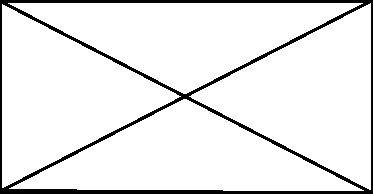
\includegraphics{filler}
    \caption{Cut. Each cycle yields a bond that must be cut.}
    \label{fig:cut}
\end{figure}

To prevent overflow, a cut index may be reused provided that it appears to the right of its last paired appearance.

An alternative to \ttt{<union>} within a sequence is the \ttt{<branch>} non-terminal (\enquote{branch}). Like union, branch joins a parent and child node through a bond. Wrapped by opening and closing parenthesis terminals (\enquote{(} and \enquote{)} respectively), branch encodes a sequence that may or may not be attached to its parent. Attachment occurs if the \ttt{<bond>} non-terminal is included. Alternatively, the sequence will be detached if the \ttt{<detachment>} non-terminal (\enquote{.}) appears. If neither \ttt{<bond>} nor \ttt{<detachment>} are present then bond to the first atom of the sequence is elided.

\begin{lstlisting}
<branch> ::= "(" ( <detachment> | <bond> )?
             <sequence> ")"
\end{lstlisting}

The third option for adding atoms within a sequence is the \ttt{<split>} non-terminal (\enquote{split}). A split is a sequence of \ttt{<detachment>} and \ttt{<sequence>} productions. The \ttt{<detachment>} non-terminal serves the same purpose as it does within a branch: to prevent the bonding to the first atom of the sequence.

\begin{lstlisting}
<split> ::= <detachment> <sequence>
\end{lstlisting}

Having defined sequence, it's now possible to define a string as an optional sequence. In other words, a Dialect string is either empty or contains a sequence. A string without a sequence encodes a molecular graph having zero nodes and zero edges.

\begin{lstlisting}
<string> ::= <sequence>?
\end{lstlisting}

\section*{Reading Strings}
\label{reading-strings}

The goal of a Dialect reader is to transform a string input into a data structure output consistent with the string's content. The output data structure can take many forms. For example, a reader can merely validate a string by returning a boolean type. A more sophisticated reader can return a molecular graph capturing all atom and bond attributes and connectivity relationships.

Dialect strings are read one character at a time starting at the leftmost character and finishing at the rightmost character. The first character sets an initial reader state, and each subsequent character causes a state transition. The cumulative application of these state transitions yields the data structure to be returned.

Readers that capture atom-atom connectivity will typically maintain a reference to a \textit{root atom}. The root atom is initially undefined. On reading the first complete \ttt{<atom>} non-terminal, the corresponding atom is constructed and set as the root atom. Subsequently processing a complete \ttt{<union>}, \ttt{<branch>}, or \ttt{<split>} non-terminal triggers three changes: (1) a child atom is constructed; (2) the child is connected to the current root atom, unless a \ttt{<detachment>} non-terminal intervenes; and (3) the root atom is replaced with the child atom.

The presence of a branch adds some nuances over a union. The leading open parenthesis terminal (\enquote{(}) signifies that the current root atom will later be re-exposed. This operation can be supported by a stack. At the start of a branch, the current root is pushed to the stack. At the end of the branch, the stack is popped and its top value is assigned as the new root atom.

\begin{figure}
    \centering
    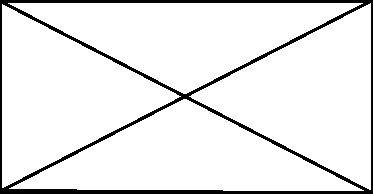
\includegraphics{filler}
    \caption{Stack for branches.}
    \label{fig:branches-stack}
\end{figure}

Further workflow adjustments can handle cuts. The necessary state can be maintained by a 100-element array. The first occurrence of a cut creates an entry in the array at the cut index consisting of the bond and the root atom. The second occurrence of a cut takes the entry at the cut index, attaching the atom in the entry to the current root atom. The two bonds spanning a cut must be \textit{compatible}. Compatibility is determined by comparing attributes using the following rules. If no rule applies to both bonds they are not compatible. It is an error to span a cut with incompatible bonds.

\begin{enumerate}
    \item An elided bond is compatible with any other bond, regardless of order or direction.
    \item A bond with a defined direction is compatible with bond having the opposite direction if \ttt{source} precedes \ttt{target} (the usual case), or the same direction otherwise.
    \item A bond without a direction is compatible with any bond having the same order.
\end{enumerate}

\begin{figure}
    \centering
    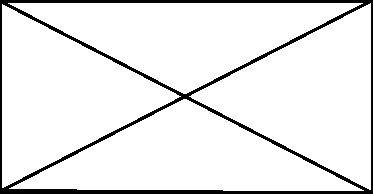
\includegraphics{filler}
    \caption{Array for cuts. The array's fixed length reflects the syntactic constraint on cut index.}
    \label{fig:cuts-array}
\end{figure}

\begin{figure}
    \centering
    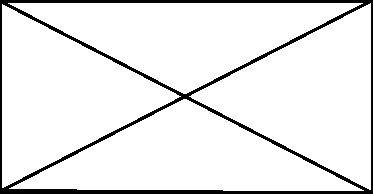
\includegraphics{filler}
    \caption{Bond compatibility. Two non-elided bonds across a cut must have compatible `order` and \ttt{direction} attributes.}
    \label{fig:bond-compatibility}
\end{figure}

One further complication applies to decoding cuts. Atomic configuration is defined in terms of the relative order of attachment of neighbors about a central atom. In the first bond of a cut pair, the neighbor atom is undefined. It won't be known until the second bond of the cut pair is found. This might only occur after the addition of several intervening neighbors. Nevertheless, the neighbor atom across the cut must precede any subsequent neighbors. This requirement can be met by a placeholder or some other mechanism that preserves the relative order of neighbor attachment. No such special treatment is needed for the second bond of a cut pair.

\begin{figure}
    \centering
    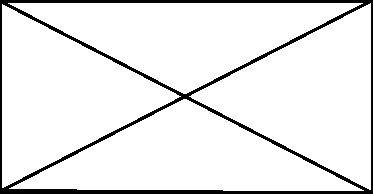
\includegraphics{filler}
    \caption{Order of attachment. A placeholder target index preserves the order of attachment.}
    \label{fig:order-of-attachment}
\end{figure}

Readers must not assume that detachment (the period terminal, \enquote{.}) implies the presence of disconnected components. This assumption is most likely to arise in the context of ad-hoc parsers using regular expressions, string matching, and the like. For example, the connected molecular graph for propane can be encoded using the string \enquote{C1C.C1}.

The use of PPBs conformation over three or more bonds. Readers must therefore report as an error any PPB not connected to an atom connected through a double bond. For example, an isolated PPB is invalid (e.g., \enquote{C/C} and \enquote{C/CC}). Beyond this check, generating (\textit{E}) and (\textit{Z}) stereodescriptors from PPBs is not a straightforward process. One approach is to first consider the parity of each double bond terminal individually. A separate step would then relate the individual terminal parities to a double bond conformation parity. This intermediate parity can then be used to perform the final conversion.

\begin{figure}
    \centering
    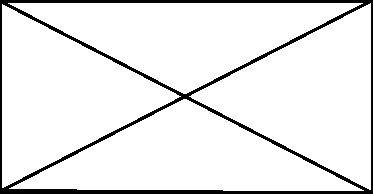
\includegraphics{filler}
    \caption{Localized configurational descriptor. Such a representation can be useful when bridging Dialect to other representations.}
    \label{fig:localized-configurational-descriptor}
\end{figure}

A reader must assume that any input string can contain errors, and take appropriate steps to report them. The most useful errors will report a specific cause. Some will also report one or more cursor indexes. The most common mandatory errors are:

\begin{enumerate}
    \item{Invalid character (position). An unexpected character was encountered. A list of acceptable characters is helpful, but not required.}
    \item{Unexpected end-of-line. Input ended unexpectedly.}
    \item{Unbalanced cut (position). A cut with a given index appears an odd number of times.}
    \item{Incompatible cut bonds (position, position). The bonds to a pair of cuts are incompatible.}
    \item{Delocalization subgraph lacks perfect matching. Before reporting this error, steps to remove unnecessarily selected atoms should be taken as described in the next section.}
    \item{Partial parity bond not allowed (position). Neither terminal of a PPB possesses a double bond. Strings such as \enquote{C/C} and \enquote{C{\textbackslash}C} contain isolated PPBs, which are invalid. A reader encountering such strings must report an error.}
\end{enumerate}

A reader may also report optional errors, including:

\begin{enumerate}
    \item{Impossible isotope. A negative implied mass number results from the atom (e.g., \enquote{[2C]}).}
    \item{Impossible valence. The valence at an atom is impossibly high (e.g., \enquote{C(C)(C)(C)(C)C}).}
    \item{Impossible charge. An atom's charge gives it an apparent negative electron count (e.g., \enquote{[C+7]}).}
\end{enumerate}

\section*{Pruning}

As noted previously, a delocalization subgraph is invalid if it lacks a perfect matching. The one exception is when a selected atom can be deleted from the delocalization subgraph through \textit{pruning}. Pruning unsets the \ttt{selected} attribute of a selected atom without corresponding promotion of any attached bonds.

An atom must be pruned if its subvalence equals zero. None of the bonds to such an atom can be promoted without altering the atom's \ttt{charge} attribute. Pruning the atom ensures the stability of its \ttt{charge} attribute, without interfering with bond promotion elsewhere. Viewed from another perspective, an atom with zero subvalence lacks unpaired electrons - at least within the narrow boundaries of the Dialect valence model. Such atoms can only form double bonds through changes to atomic charge. 

If a selected atom bears a non-zero \ttt{charge} attribute, subvalence is computed using the isoelectronic element's default valences. For example, a selected nitrogen atom with a charge of +1 would use the default valences for carbon. A selected phosphorous atom with a charge of -1 would use the default valences of sulfur. And so on. If no default valences are found in this way (e.g., \enquote{[c+2]}), a reader must generate an error. Writers must not encode such atoms.

\begin{figure}
    \centering
    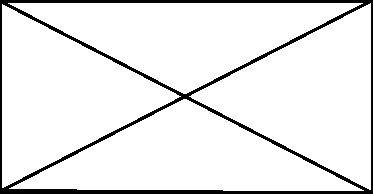
\includegraphics{filler}
    \caption{Gratuitous selection.}
    \label{fig:gratuitous-selection}
\end{figure}

Pruning becomes necessary in cases of gratuitous atomic selection. This occurs whenever style, tradition, or convenience overrides necessity. Consider a string representing furan in which all atoms are selected (e.g., \enquote{c1ccco1}). Selecting any atom is unnecessary because furan does not exhibit DIME. But selecting the oxygen atom is particularly unnecessary because it lacks an unpaired electron and so will never lead to DIME. It is nevertheless convenient to select the carbon atoms because all bonds can then be elided. The resulting representation (e.g., \enquote{c1cccO1}) leads to a delocalization subgraph with a perfect matching and hydrogen counts consistent with the original encoding.

Writers are encouraged, but not required, to avoid gratuitous atom selection. Readers, however, must always be prepared to prune.

\section*{Writing Strings}

Whereas a reader transforms a string into a data structure, the goal of a writer is the opposite: to transform a data structure into a valid string. This data structure will most commonly take the form of a molecular graph, but other forms are possible. Although a graph itself could be used as the basis for an input representation, a more primitive representation such as an adjacency list could also be used. For practical reasons, the input data structure is likely to resemble the output from a reader. Such an arrangement makes it possible to encode and decode strings with minimal intermediate translation.

Regardless of the form taken by the input data structure, it must be traversable in \textit{depth-first} order. A depth-first traversal operates over a set of nodes bound by a set of connectivity relationships, which are typically edges. Traversal proceeds by successively replacing each node as the center of focus, or root. Each new root is selected from the untraversed neighbors of the current root. Iteration eventually selects all nodes, at which point the traversal ends.

\begin{figure}
    \centering
    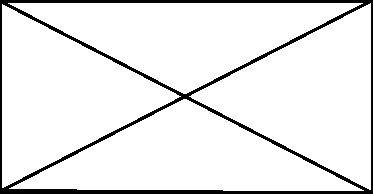
\includegraphics{filler}
    \caption{Depth-first traversal.}
    \label{fig:depth-first-traversal}
\end{figure}

A writer intercepts the depth-first traversal of an input data structure to write node and edge representations. The \ttt{<atom>} and \ttt{<bond>} non-terminals are used for this purpose. There are no requirements around style. For example, it's equally valid to represent the carbon atom of methane using either implicit or virtual hydrogens (e.g., \enquote{C} or \enquote{[CH4]}). Single bonds may be elided or not. Similarly, the DS may or may not be empty. Although an organization may seek to standardize certain styles of string output, any syntactically-valid string must be considered valid by a reader.

The presence of branches within an input data structure is encoded via the \ttt{<branch>} non-terminal. A useful tool for this purpose is a \ttt{stack}. A stack is a data structure that allows items to be added individually and removed (\enquote{popped}) in the reverse order of addition. A writer begins by pushing the current branch onto the stack and extending it. When a new branch is encountered, it is pushed to the stack and extended. When the branch terminates, the current branch is popped and its contents are appended to the stack's new top item.

\begin{figure}
    \centering
    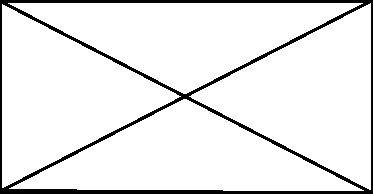
\includegraphics{filler}
    \caption{Stack for branch assembly.}
    \label{fig:branch-stack}
\end{figure}

Cycles are encoded using the \ttt{<cut>} non-terminal. This one- or two-digit integer replaces one terminal of a cycle closure bond. The challenge is to unambiguously supply these integers while allowing re-use to avoid overflow. This can be accomplished with a \textit{pool}. A pool is a data structure that yields a numerical index given an ordered pairing of atomic indexes. The numerical index will not be re-issued until the pool receives the corresponding reversed pairing.

\begin{figure}
    \centering
    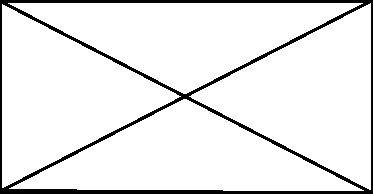
\includegraphics{filler}
    \caption{Pool for assigning cut indexes.}
    \label{fig:pool}
\end{figure}

A pool can be used by a writer in the following way. The presence of a cycle during depth-first traversal is indicated by an atom that has already been traversed. On encountering a cycle, a writer requests an index from the pool, submitting the corresponding atomic indexes as an ordered pair. Later, the same bond must be reversed in the reverse direction. When it is, the writer once again requests an index, but this time using a reversed pairing. Doing so yields the same index, while simultaneously freeing it for later use.

The encoding of cuts is likely to pose special challenges for writers. For a cut across a PPB, care must be taken to report the correct parity. Consider \textit{trans}-cyclooctene. The correct encoding accounts for the reverse in parity at the left-hand side (e.g., \enquote{C{\textbackslash}1C=C/CCCCC/1}). Moreover, the double-encoding of the PPB bond type can lead to inconsistencies that must be reported by a reader (e.g., the invalid string \enquote{C/1C=C/CCCCC/1}). Such errors can be avoided by encoding the bond type of one side or the other side of a cut, but not both. (e.g., \enquote{C{\textbackslash}1C=C/CCCCC/1} or \enquote{C1C=C/CCCCC/1}). A cut across a bond attached to an atom with a stereodescriptor must take bond ordering into consideration. For example, the two strings \enquote{O[C@H]1NC1} and \enquote{O[C@H](C1)N1} encode the same configuration, but the string \enquote{O[C@H](N1)C1} encodes the \textit{opposite} configuration. 

\begin{figure}
    \centering
    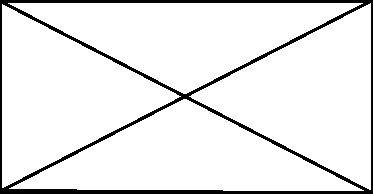
\includegraphics{filler}
    \caption{Difficult cuts.}
    \label{fig:difficult-cuts}
\end{figure}

The presence of conformational restriction about a double bond presents a special challenge to writers. Few other molecular graph systems distribute a conformation descriptor over multiple individual bonds the way that PPBs does. Instead, descriptors are more likely to be localized at the double bond. Producing the necessary PPBs from a descriptor localized at the double bond is likely to be non-trivial. An approach to the reverse problem was presented previously (\nameref{reading-strings} section). That approach can also be adapted to the reverse problem.

\begin{figure}
    \centering
    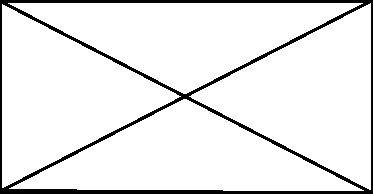
\includegraphics{filler}
    \caption{Writing partial parity bonds through a localized conformation descriptor.}
    \label{fig:writing-ppb}
\end{figure}

Writers should carefully weigh the non-negligible costs of atom selection. Algorithms for selection are likely to involve the perceptions of cycles, and could exhibit superlinear time complexity. Often, a reader must perform a global deselection to arrive at a localized valence bond representation, which at the very least requires pruning and a maximal matching procedure. In this sense atom selection imposes two sets of costs: one on the writer and the other on every subsequent reader forever into the future.

Writers must ensure that all selected atoms can be deselected. Consider pyrrole, erroneously encoded with a selected nitrogen atom (e.g., \enquote{n1cccc1}). The nitrogen atom can not be pruned because of its subvalence is 1 (3 - 2). The DS therefore contains all five atoms and all five bonds. A perfect matching does not exist. A reader receiving such a string must report an error. To avoid this outcome, a writer can consume the subvalence by adding a virtual hydrogen (e.g., \enquote{[nH]1cccc1}). The subvalence of nitrogen in this case is zero, so the atom can be pruned. Doing so leaves a DS with four nodes, four edges, and a perfect matching. Readers will consider the string valid. Nevertheless, the larger question of gratuitous selection remains.

\section*{Compatibility}

For maximum compatibility with existing software, Dialect was designed as a \textit{language subset} of SMILES. A language subset contains some of the syntax and semantics of its parent language, but adds none of its own. In principle this means that a feature present in Dialect should also be present in SMILES. Conversely, a feature present in SMILES may or may not also be present in Dialect.

Language subsets have ample precedent in computer science. A well-known example is MISRA C~\cite{misraC}, a subset of the C programming language that aims to eliminate \enquote{known undefined or otherwise dangerous behavior}~\cite{hatton:2007}. Another example is the subset of JavaScript described by Crockford whose purpose is to \enquote{chip away at the features that are not beautiful until the language's true nature reveals itself.}~\cite{crockford:2008}. Language subsets arise for two main reasons. First, designing a language presents many opportunities to introduce errors small and large. Second, popular languages inevitably bring with them many users with diverse problems that demand new features. Some of these features cause future problems of their own. A language subset can improve both situations by eliminating the most problematic features.

Although similar considerations apply to SMILES, its case is different in one important way: SMILES was never publicly described with high precision. Overviews of the language have been published by both Weininger and Daylight. But the kind of technical documentation suitable for software development was never made public. Both the OpenSMILES and SMILES+ initiatives cite this shortfall as motivation.

Nevertheless, several SMILES software implementations have been released as noted previously. Each one represents its own unique set of decisions about how to reduce the published broad SMILES descriptions to a specification detailed enough for software development. Some implementations have themselves been reverse-engineered for clues. The Daylight implementation in particular is sometimes invoked as a de facto SMILES specification. Unfortunately, access to this implementation is restricted by commercial licensing, as is the case with several SMILES implementations. Moreover, reverse engineering is unlikely to address every question because of the vast search space embodied by SMILES. Although some implementations are released under Open Source licenses, they are neither authoritative nor unanimous in their interpretations.

A publicly-available and precise subset of SMILES would offer a new way to address the problem. If sufficiently constrained, the subset should be interpretable by all existing software without modification. Moreover, most strings written by existing software would be interpretable by software based on the language subset. Because its description would be both public and precise, the language subset could serve as the basis for many implementations with strong consensus around both syntax and semantics.

Unfortunately, the choice of the Dialect base language is fraught with difficulty on technical, historical, and cultural grounds. Simply put, the term \enquote{SMILES} has come to mean different things to different people. To some, SMILES is the language defined in public documentation. To others, SMILES is the Daylight implementation source code. Some may view SMILES as the collective definitions contained in both published documents and all software. To others, SMILES isn't even definable.

These problems can be avoided by considering as a base language not SMILES itself, but a \textit{protolanguage}. A protolanguage is a hypothetical language from which a family of languages can be derived. A suitable SMILES protolanguage would ideally contain all of the features consistent with the many ways in which the term \enquote{SMILES} is used today.

Accordingly, Dialect's base language is \enquote{ProtoSMILES,} a SMILES protolanguage. ProtoSMILES was developed through a process of elimination that started with every SMILES document ever published and every SMILES software implementation, Open Source or not. The field was narrowed through two limitations: (1) the source must be authoritative; and (2) the source must be publicly accessible. In this context, authoritative means that the source was created by either Weininger himself or Daylight. They alone can speak most authoritatively about what SMILES is. The requirement for public accessibility ensures that, even if inconvenient, claims of compatibility can be tested. The following documents were identified as candidate ProtoSMILES sources:

\begin{itemize}
    \item Weininger's report to the US Environmental Protection Agency (\enquote{The Article})~\cite{anderson:1987}.
    \item Weininger's original publication (herein \enquote{The Article})~\cite{weininger:1988}.
    \item Weininger's 2003 book chapter, revised in 2008 (\enquote{The Book Chapter})~\cite{weininger:2003}.
    \item An online manual maintained by Daylight (\enquote{The Manual}).
    \item The Daylight's toolkit, which implements a SMILES reader and writer (\enquote{The Toolkit})~\cite{daylightToolkit}.
\end{itemize}

The Toolkit was eliminated for three reasons. First, its source code is not available, forcing an indirect reverse-engineering approach to language definition. Second, as a product of the company Weininger started, the Toolkit is likely to recapitulate the other sources. Third, as a commercial product without source code, the Toolkit may not always be available in the future.

The Report was eliminated mainly because the contents of this older document contradict the three remaining sources. For example, The Report contains no mention of bracket syntax, using markedly different notation instead. The report also supports unusual characters including the exclamation mark (\ttt{!}). Semantically, The Report supports \enquote{special states} for nitrogen-containing atoms.

The Manual was disregarded as a ProtoSMILES source because it merely recapitulates content already present in The Paper and The Book Chapter. Removing this source simplifies the construction of ProtoSMILES without changing its definition. A secondary consideration was the possibility that updates to this web page could change the meaning of ProtoSMILES. However, web archives indicate that neither styling nor content of the Manual have changed in at least ten years.

The only remaining sources are The Paper and the Book Chapter. Therefore, these two works collectively define ProtoSMILES. The remainder of this section compares and contrasts ProtoSMILES with Dialect. The main difficulty with this approach is that the works defining ProtoSMILES not only contradict each other in some ways, but they also contradict themselves internally. These contradictions will be noted when meaningful.

The Book Chapter defines a fixed set of element symbols which even at the time of publication was obsolete~\cite[p.~83]{weininger:2003}. The symbol for element 105 is given as Ha (Hahnium), despite IUPAC's resolution of this naming controversy in favor of the symbol Db (Dubnium) years prior~\cite{sageson:1997}. Accordingly, Dialect disallows the symbol Ha. To support the full set of currently-named transuranium elements, Dialect adds the symbols: Db; Sg; Bh; Hs; Mt; Rg; Cn; Nh; Fl; Mc; Lv; Ts; and Og. Moreover, Dialect explicitly accepts all future element symbols approved by IUPAC. The addition of these element symbols means that Dialect can't be considered a strict subset of SMILES. The alternative would, however, leave dialect without the ability to express every kind of IUPAC-recognized element.

The Article implies that comma (\ttt{,}) is either an element symbol or a valid SMILES character: \enquote{This subset uses only the symbols H, C, N, O, P, S, F, Cl, Br, I, and (,) and digits, with the following four rules...}~\cite[p.~33]{weininger:1988}. The comma character is explicitly disallowed in Dialect.

The Book Chapter defines a recursive grammar for branching which, perhaps without the knowledge of the author, allows sequentially nested parentheses~\cite[p.~86]{weininger:2003}. Dialect disallows such constructs (e.g., \enquote{*((*))*} and \enquote{*(((*)))*}).

\enquote{Reaction SMILES} is an extension described in the Book Chapter~\cite[p.~89]{weininger:2003}, but disallowed in Dialect. Specifically, the greater than symbol (\ttt{$>$}) is not a valid Dialect character. This precludes strings such as \enquote{*$>$$>$*} in Dialect. Furthermore, Dialect lacks the \enquote{map} attribute, used for atom-atom mapping in reactions, and its accompanying syntax.

Dialect only supports two stereodescriptors, encoded with the terminals \enquote{@} and \enquote{@@.} The Book Chapter provides a recursive grammar for stereodescriptors that allows multi-symbol descriptors such as \enquote{@@@} and \enquote{@@@@}~\cite[p.~94]{weininger:2003}. The book chapter also discusses non-tetrahedral descriptors including \enquote{@AL1,} \enquote{@AL2,} \enquote{@1,} and \enquote{@SP1.} None of these are supported by Dialect. Nor does Dialect support the application of tetracoordinate stereodescriptors to odd cumulenes as described in the book chapter. Although some of these forms of configuration are supported today, it's unusual to find them all supported. The reason is simple: in the context in which Dialect will most often used, these forms of stereochemistry are rare. To support them burdens implementors with little payoff.

ProtoSMILES supports the concept of \enquote{aromatic bond} (\enquote{:}), but Dialect does not. Despite clear inclusion within the syntax of ProtoSMILES, no precise guidance on using this feature is provided. The Book Chapter notes \enquote{Adjacent atoms without an intervening bond symbol are connected by a valence-dictated bond (typically a single or aromatic bond) \enquote{-} (single) and \enquote{:} (aromatic) bond symbols may always be omitted on input}~\cite[p.~85]{weininger:2003}. This passage implies that aromatic bonds serve no purpose. Accordingly, Dialect does not allow them and the syntax does not include the colon symbol (\ttt{:}).

Along these lines, Dialect does not recognize atoms bearing either arsenic (As) or selenium (Se) as selectable. Doing so would increase the complexity of the language unnecessarily. Although The Paper implies selectability (\enquote{Elements other than C, N, O, P, S, As, and Se are not yet dealt with in an aromatic context.})~\cite[p.~35]{weininger:1988}, default valences for the latter two atoms are not provided. Even if they were, the elements As and Se must be bracketed. As such, special rules for handling them in the context of pruning would be required. Moreover, molecules bearing the elements As or Se are often made \enquote{aromatic} unnecessarily in SMILES. Finally, allowing the selection of atoms bearing As or Se does nothing to address molecules with atoms bearing silicon, germanium, tin, or other heavy main group elements that may be discovered in the future to participate in DIME.

It's unclear whether ProtoSMILES allows a virtual hydrogen count on hydrogen itself. The Article implies that the element symbol H (hydrogen) must not have an implicit hydrogen count when used within a bracket sequence (\enquote{There are few exceptions to the hydrogen-suppression convention, the most obvious being specification of a proton, [H+], and molecular hydrogen, [H][H].})~\cite[p.~34]{weininger:1988}. If so, the author may have erroneously believed that parsers would be incapable of processing strings encoding bracket hydrogen with a virtual hydrogen count (e.g., \enquote{[HH]}). The Book Chapter appears to reiterate this view, noting that \enquote{explicit hydrogen specification is required} in the case of \enquote{hydrogens connected to other hydrogens, e.g. [H][H], molecular hydrogen}~\cite[p.~97]{weininger:2003}. To be clear, Dialect supports any valid virtual hydrogen count on hydrogen itself (e.g., \enquote{[HH]} and \enquote{[HH2]}). Subject to interpretation of the original literature, this feature may or may not render Dialect a superset of SMILES.

ProtoSMILES ascribes ambiguous meaning to detachments. As noted in the Book Chapter, \enquote{... In terms of the valence model being represented, the dot literally represents a bond of formal order zero: the atoms on either side of the dot are explicitly not bonded to each other.}~\cite[p.~88]{weininger:2003}. Other statements appear to contradict this statement. To be clear, the state of not being bonded and the state of having a zero-order bond are not necessarily equivalent~\cite{clark:2011}. Dialect explicitly disallows the zero bond order interpretation of detachments and the dot character.

ProtoSMILES assigns no explicit upper or lower bounds to numerical atomic attributes. These boundaries are nevertheless crucial for implementors, who seek the data types necessary to prevent underflow and overflow. For this reason, Dialect sets both upper and lower bounds on the following atomic attributes: isotope (0 $\leq$ value \textless 1000); charge (-10, \textless value \textless 10); and hydrogens, 0 $\leq$ value \textless 10). Although it might be argued that lower bounds on physical quantities such as isotope and hydrogen count should be implicit, the lack of precision forces implementors to improvise, which can lead to divergent behavior. ProtoSMILES places no upper bound on the charge notation (e.g., \enquote{++} and \enquote{+++}) and their corresponding negative forms: \enquote{The SMILES program also recognizes constructions of the form [Fe+++] as being synonymous with the form [Fe+3]}~\cite[p.~32]{weininger:1988}. Due to their redundancy, Dialect disallows duplicated plus and minus characters (\ttt{+} and \ttt{-}, respectively) within bracket atoms.

Dialect provides a few semantic clarifications not fully addressed in ProtoSMILES. A detailed algorithm for determining implicit hydrogen count is provided, together with the required valence table. Unlike ProtoSMILES, Dialect explicitly considers the case of computing implicit hydrogen counts on selected atoms. Dialect also provides detailed algorithms, absent in SMILES, for selection and deselection. These are based in graph theory rather than the ambiguous and overloaded chemical concept of \enquote{aromaticity} used in ProtoSMILES. Uniquely, Dialect introduces the concepts of \enquote{pruning} and \enquote{gratuitous selection.} ProtoSMILES does not specify those bonds that can be promoted during deselection, but Dialect does. ProtoSMILES does not restrict partial parity bonds to those atoms also possessing at least one double bond, whereas Dialect does. Finally, Dialect syntax is based on a formal grammar and tooling rooted in decades of computer science research, whereas ProtoSMILES syntax is based for the most part on imprecise natural language descriptions.

Dialect also resolves some internal contradictions within ProtoSMILES. The Article reports the only default valence for nitrogen as three (p. 34)~\cite[p.~34]{weininger:1988}, whereas the Book Chapter reports two default valences: 3 and 5~\cite[p.~84]{weininger:2003}. Dialect uses the latter default valences. Atoms whose \ttt{hydrogens} attribute may be set to \ttt{Implicit} (\enquote{the organic subset}) are reported in the Article as: B; C; N; O; P; S; F; Cl; Br; and I~\cite[p.~32]{weininger:2003}. However, an example later in the Article indicates that the string \enquote{Hn1cccc1} with its unbracketed hydrogen valid~\cite[p.~35]{weininger:1988}. Dialect explicitly rejects strings containing unbracketed hydrogen atoms. On the topic of atom selection (\enquote{aromaticity}), The Article implies that selected atoms must be part of a cycle: \enquote{To qualify as aromatic, all atoms in the ring must be sp2 hybridized and the number of available 'excess' $\pi$ electrons must satisfy Hückel's 4{\textit{N}} + 2 criterion}~\cite[p.~34]{weininger:1988}. The Book Chapter, however, presents two examples of valid strings that do not encode cycles (\enquote{cc} and \enquote{cccc})~\cite[p.~85]{weininger:2003}. Consistent with the latter view, Dialect explicitly allows the selection of atoms regardless of cycle membership.

\begin{table}
\begin{minipage}{\textwidth}
\renewcommand*\footnoterule{}
    \caption{Some differences between ProtoSMILES and Dialect.}
    \centering
    \begin{tabular}{p{0.50\linewidth} p{0.20\linewidth} p{0.15\linewidth}}
        \hline
        Feature & ProtoSMILES\footnote{Values of \enquote{maybe} indicate ambiguous and/or contradictory statements in the authoritative sources.} & Dialect \\
        \hline
        element symbol Ha & yes & no \\
        element symbols Db; Sg; Bh; Hs; Mt; Rg; Cn; Nh; Fl; Mc; Lv; Ts; and Og & no & yes \\
        future element symbols approved by IUPAC & no & yes \\
        comma symbol (\enquote{,}) & maybe & no \\
        multiple branching (e.g., \enquote{*((*))*}) & yes & no \\
        reactions using greater than symbol (\ttt{>}) & yes & no \\
        atomic \enquote{map} attribute & yes & no \\
        extended stereodescriptors (e.g., \enquote{@@@} and \enquote{@OH1}) & yes & no \\
        use of stereodescriptors on odd cumulene centers & yes & no \\
        virtual hydrogen count on hydrogen (e.g., \enquote{[HH]}) & maybe & yes \\
        detachments are bonds of \enquote{formal order zero} & maybe & no \\
        unbounded numerical atomic properties & yes & no \\
        nitrogen default valence includes 5 & maybe & yes \\
        unbracketed hydrogen atom & maybe & no \\
        acyclic atom selection & maybe & yes \\
        atoms with elements As and Se are selectable & yes & no \\
        non-elided bonds may be promoted during selection & maybe & no \\
        isolated partial parity bond & yes & no \\
        repeated charge notation (e.g., \enquote{++} and \enquote{+++}) & yes & no \\
        aromatic bond (\enquote{:}) & yes & no \\
        \hline
    \end{tabular}
    \label{table:feature-comparison}
\end{minipage}
\end{table}

With only one clear-cut exception, Table~\ref{table:feature-comparison} shows Dialect to be a subset of ProtoSMILES. The exceptional case deals with the validity certain transfermium element symbols already recognized by IUPAC and to be recognized in the future by Dialect. Ambiguous exceptions include those for which the ProtoSMILES column feature support is uncertain (\enquote{maybe}) but the Dialect column is affirmative (\enquote{yes}). If ProtoSMILES support tends toward \enquote{no,} then support by Dialect would break out of the ProtoSMILES subset. There are three such cases: hydrogen having virtual hydrogens (e.g., \enquote{[HH]}); whether or not the default valence of nitrogen includes the value five; and whether or not ProtoSMILES recognizes acyclic \enquote{aromatic} atoms as valid.

\section*{Discussion}

Dialect's main advantage as a molecular serialization format is high information density. The most common atom types can be represented with just one character. The worst case atom, using every available atomic attribute, requires 14 characters. The most common bond types can be encoded implicitly. In the worst case one character per bond is required.

These metrics compare favorably with alternatives. Consider the molfile (V2000) format. 32 characters per atom are required in the best case, and 51 characters in the worst. All bonds, regardless of type, require between nine and 12 characters. Atomic charges and isotopes typically require additional characters.

The information density of Dialect strings makes them attractive for several applications. In memory-constrained environments such as those found on handheld devices and network serialization, many more Dialect strings can be present than alternative encodings. In-memory structure search over large collections becomes feasible. Because a Dialect string often fits within one line on a terminal, it can be used for data entry in manual interactive shells such as a real-eval-print loops (REPLs) or notebooks.

Another advantage is lossless serialization and deserialization. The line notation InChI might appear to compete with Dialect in this sense. The authors of InChI have noted that InChI is not a solution to the molecular serialization problem but rather an identifier.\cite{heller:2015} The reason presumably lies with the fact that both serialization and deserialization require intimate knowledge of the InChI canonicalization algorithm. To date, no third-party reader or writer of InChI has ever been released.

Despite its information density, Dialect can faithfully encode and decode most of what chemists would consider \enquote{organic molecules.} This is evidenced by the widespread presence of Dialect strings within large, public-facing databases such as PubChem,\cite{kim:2016} ChEMBL,\cite{gaulton:2012} ChEBI,\cite{degtyarenko:2007} and others.

Dialect's compact representation requires some tradeoffs regarding expressiveness. Extended bonding beyond the delocalization subgraph is not supported. This limitation excludes many types of molecule, including organometallics and delocalization-\-stabilized ions. Zero-\-order bonds are not supported, making it difficult to accurately encode coordination complexes. Only four-\-coordinate, tetrahedral stereocenters can be encoded, excluding many forms of chirality, including helical chirality, all forms of non-\-tetrahedral stereochemistry, and lone-\-pair tetrahedral centers. Conformational restrictions beyond the isolated double bond are not supported, which excludes important molecules such as those exhibiting atropisomerism. Other formats such as CDXML and molfile support enhanced stereochemical features enabling the differentiation of various kinds of partial stereochemical information, but Dialect does not.

Broader expansion of Dialect's capabilities could be possible through \textit{metaformats}. A metaformat embeds one or more Dialect strings within a surrounding serialization format. For example, two- or three-dimensional coordinates could be associated with each atom through a metaformat that includes a dictionary mapping atomic index to coordinate. Collections of atoms or bonds could likewise be encoded to replicate the enhanced stereochemistry features of other formats. And so on. However, the utility of such extensions should be weighed against Dialect's main value proposition: high information density. An application attempting to use a verbose metaformat may benefit from adopting better-suited format instead.

Setting aside the many technical and usability issues a metaformat would raise, versioning is likely to play an important role. Dialect itself lacks any mechanism to convey the concept of version. This stands in contrast to InChI, which not only encodes a version identifier, but has done so from its first release. Adding a version identifier would, unfortunately, break compatibility with the large number of existing SMILES software. Metaformats offer an opportunity to address this limitation.

The most noteworthy feature of Dialect is its compatibility with SMILES. Contemporary SMILES implementations will be able to read and write Dialect strings --- at least to a point. Incompatibilities will arise from two main sources: (1) those features of SMILES that Dialect has deliberately omitted; and (2) those aspects of the SMILES language that are incompletely-specified, ambiguous, or self-contradictory.

The availability of a minimal yet highly functional, fully-specified core language offers many opportunities to improve data quality. One of the most important will be an open reference implementation, the design and source code of which will be discussed later. A freely-available reference implementation in turn makes automated validation suites possible. These suites can improve data quality by reporting syntax and semantic differences among implementations, preferably before release. A reference implementation taken together with the guidelines for readers and writers in this paper should make it possible to write software that conforms to a very high level of precision, regardless of programming language or paradigm. Given verified implementations, performance optimizations can be considered. The existence of a core language specification should also aid standardization efforts, either for Dialect itself, or SMILES. Finally, the development of better line notations is only possible given a thorough understanding of the scope and limitations of existing options. Here, metaformats could offer a bridge from the present to the future.

\section*{Conclusion}

This paper describes Dialect, a subset of the widely-\-used SMILES line notation. Dialect's features are detailed at four levels: constitution; delocalization; conformation; and configuration. Constitutionally, Dialect can encode any molecule conforming to the valence bond model. In the event of undesired symmetry artifacts due to delocalization, Dialect offers a mitigation based in graph theory. Conformational isomerism of alkenes is supported by partial parity bonds. The configurations of tetracoordinate, stereogenic atoms are encoded through the use of a parity enumeration and conventions around its use.

Dialect's syntax is described in detail through a formal grammar. This method concisely summarizes the complete set of strings that could be considered syntactically valid Dialect representations. The formal grammar was deliberately structured to be used either directly with an automated parser generator or with a hand-written recursive-descent parser.

The complete set of operations needed to interpret Dialect's syntax semantically are described in detail. This is a crucial component of the language's definition because Dialect achieves its information density largely by favoring convention over encoding. As an aid to difficult cases, guidelines for readers and writers are included.

As a subset of SMILES, Dialect can be used with a wide range of SMILES software today. In this sense, Dialect may seem to offer nothing new or even of value. However, Dialect has been defined at a level of detail that SMILES never was. This difference makes it possible to use Dialect in unique ways. Open reference implementations and validation suites can now be developed and deployed. Families of extensions can be built, each one based on the same unambiguous foundation. Formal standardization becomes more feasible given detailed reference material on which to draw. Finally, it is only through the clear demarcation of boundaries that the frontier becomes visible.

\clearpage
\printbibliography

\end{document}